\subsection{Introduction}

An increasing number of atmospheric dynamical cores are being developed to maximize efficiency on massively parallel systems, paving the way towards regionally high-resolution, or even globally high resolution simulations \citep[approximately $\Delta x = 50$ km or less;][]{Z2014QJRMS,HETAL2016JCLIM,LetAl2018JAMES}. Incorporating these advances into Atmospheric General Circulation Models (AGCMs) requires the development of physical parameterizations appropriate for the diversity of grid configurations that dynamical cores are now able to support, referred to as scale-aware physics. The most common approach to understand and develop scale-aware physics has been through the lens of limited area, cloud resolving simulations. In filtering cloud resolving solutions to some target, lower resolution grid resembling an AGCM, and studying how the filtered moments vary as a function of target grid resolution, one may develop a more general relationship between resolved and unresolved scales. While this approach is likely necessary for developing scale-aware physics, it is not sufficient. The equations of motions of motion have inherent scale dependencies \citep{O1981JAS,WETAL1997MWR,PG2006JAS,JR2016QJRMS}, and the resolved dynamics act accordingly to the scales a grid is able to support. Scale-aware physics should also accommodate these dependencies.

The sensitivity of the Community Atmosphere Model (CAM) to horizontal resolution is well documented over the last few decades \citep{KW1991JGR,WETAL1995CD,W1999T,W2008TELLUS,LETAL2011TELLUS,RJ2011MWR,RETAL2012ASL,OETAL2013JCLIM,RETAL2013JCLIM,ZetAl2014JCb,LETAL2015JCLIM}. The general tendency is for the atmosphere to become drier and less cloudy, the deep convection scheme less active and the magnitude of resolved vertical motion greater with increasing resolution. \cite{HR2017JCLIM,HR2018JAMES} analyzed a set of CAM simulations and found that resolved updrafts dominate the vertical velocity field of tropical convecting systems at resolutions typical of present day global models ($208.5 km \geq \Delta x \geq 27.8 km$). The scale of resolved updrafts are collocated in the horizontal with the buoyancy produced by grid-scale clouds (also referred to as stratiform clouds in the literature), and are grid limited, conforming to the effective resolution of the model ($5-10\Delta x$). Assuming that there is a characteristic buoyancy length scale associated with a grid resolution, and it is proportional to $\Delta x$, the ratio of the vertical velocity scale of that grid resolution $W$ to a high-resolution reference simulation $W_{ref}$ is:
\begin{equation}
\alpha = \frac{W}{W_{ref}} = \frac{\Delta x_{ref}}{\Delta x} , \label{eq:eq6-1}
\end{equation}
where $\Delta x_{ref}$ is the grid-spacing of a high-resolution reference, and it is assumed that the magnitude and height scale of the buoyancy is unchanged or compensating across resolutions. The physical interpretation of equation~\ref{eq:eq6-1} is a rising column of buoyancy creates a low pressure perturbation of similar horizontal scale in its wake, and this pressure gradient scales like $\Delta x^{-1}$, facilitating convergence into the pressure minimum and the resultant vertical velocity also scales like $\Delta x^{-1}$. While \cite{HR2017JCLIM} found that equation~\ref{eq:eq6-1} over-predicted the change in vertical velocity across resolutions in their aqua-planet simulations, \cite{HR2017JCLIM} discovered that this over-prediction was at least in-part, due to time-truncation errors arising from too small a physics time-step, $\Delta t_{phys}$, in the higher resolution simulations.

In this study, it is shown that through scaling $\Delta t_{phys}$ such that time-truncation errors are relatively small \citep[Appendix A][]{HETAL2019JAMES}, the scaling of equation~\ref{eq:eq6-1} explains the change in the magnitude of the vertical velocities across resolutions in an aqua-planet configuration using CAM. The implications of the scaling are that for a doubling of the resolution, CAM can simulate the same resolved mass flux in half the area. The grid-scale cloud fraction and ascending regions are then confined to a smaller area, and the area and magnitude of subsiding motion increases with resolution. The greater subsiding motion dries and stabilizes the atmosphere, reducing the frequency the deep convection scheme is triggered. Section $6.2$ describes the model and experimental design, section 6.3 presents results and section 6.3 provides the conclusions.

\subsection{Methods}

\subsection{Results}

The probability density function (PDF) of negative, or upward vertical pressure velocities $\omega$ in the aqua-planets are shown in Figure~\ref{fig:2pdf}a. The magnitude of upward $\omega$ increases in a monotonic way with resolution, with positive, or downward $\omega$ behaving similarly (not shown). The PDF's may be scaled to the high-resolution $ne120$ resolution, through $P(\omega)_s = \alpha P (\omega / \alpha)$, where $\alpha$ is the scale factor of equation~\ref{eq:eq6-1}. The scaled PDFs all line up on top of the high-resolution reference (Figure~\ref{fig:2pdf}b); equation~\ref{eq:eq6-1} explains the variation in vertical velocity across resolutions to first order. 

\begin{figure}[t]
\begin{center}
\noindent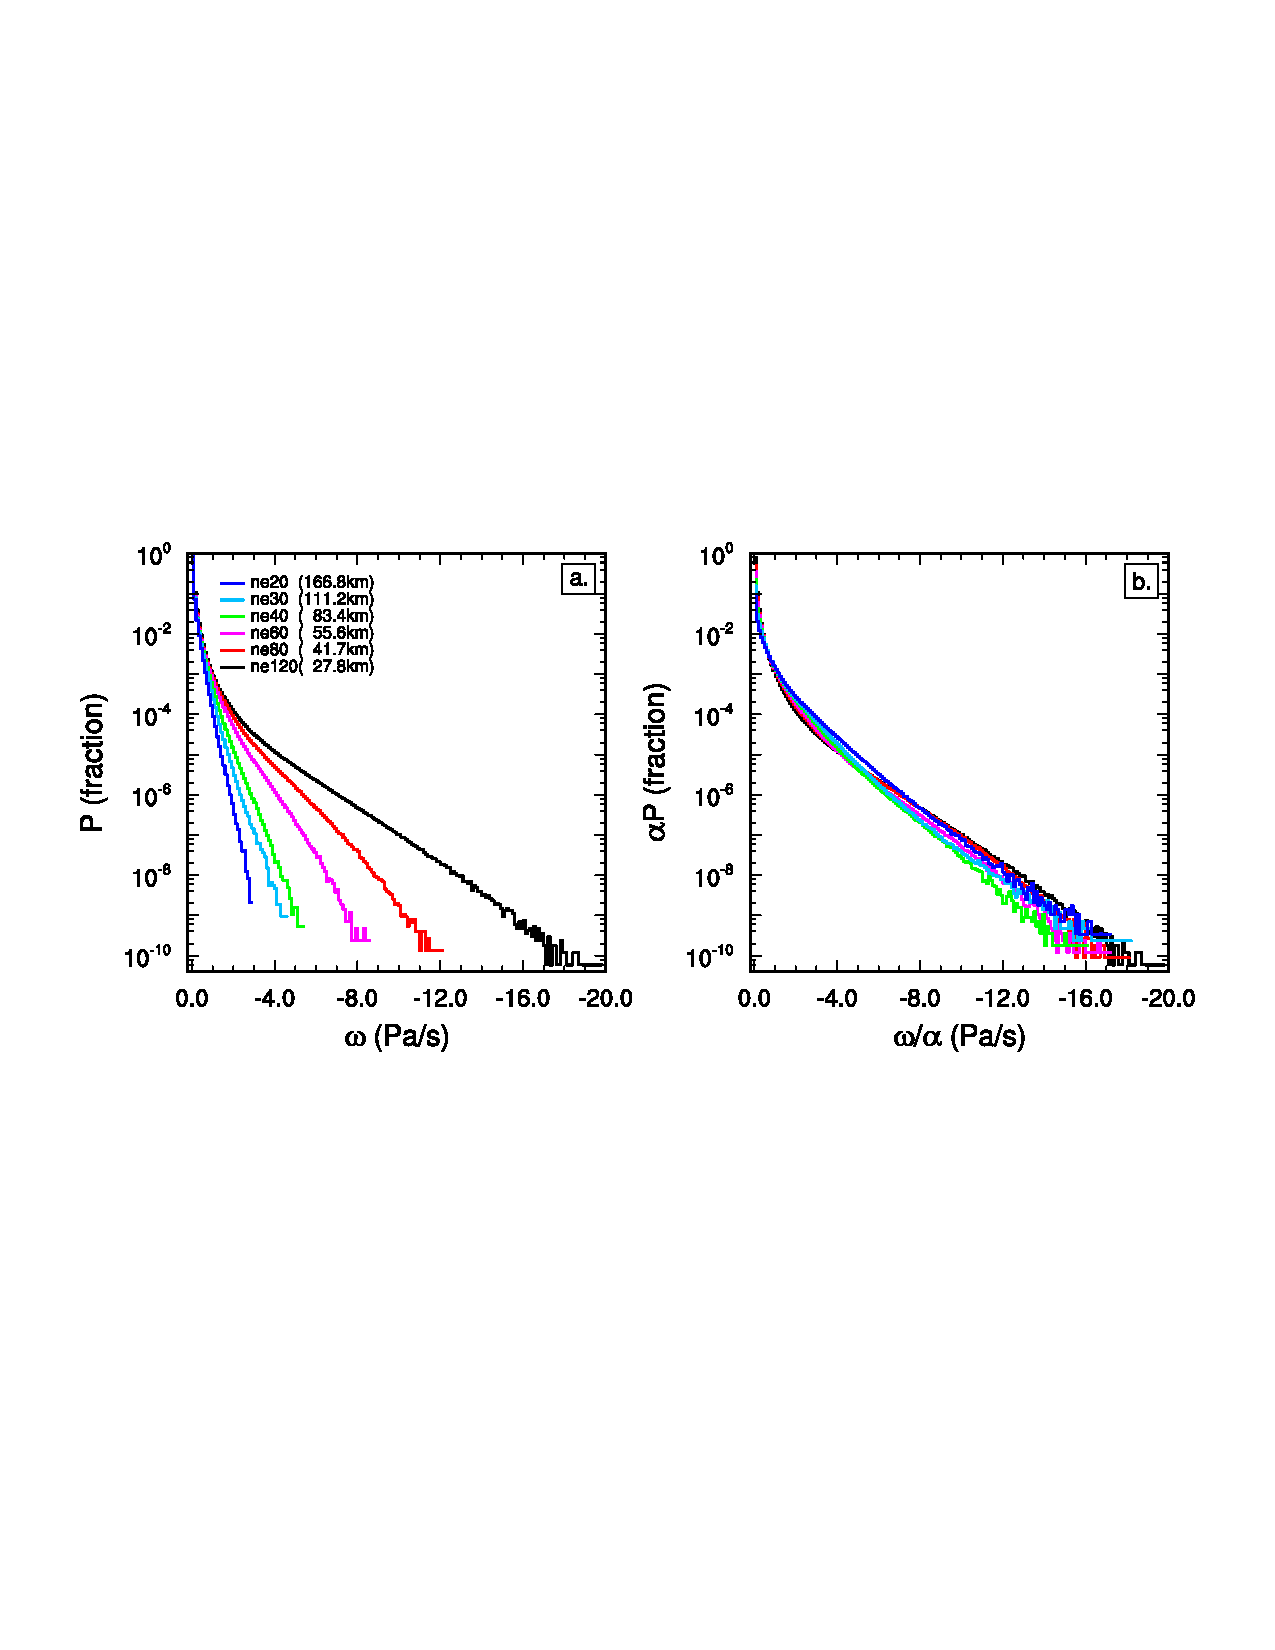
\includegraphics[width=30pc,angle=0]{chapter6/temp_2pdf.pdf}\\
\end{center}
\caption{}
\label{fig:2pdf}
\end{figure}

The impact of the changing vertical velocity field on the global mean state can be understood through decomposing the mass weighted global mean $\omega$ into upward and downward components,
\begin{equation}
\overline{\langle \omega \rangle} = \overline{\langle f_{u} \rangle} \, \overline{\langle \omega_{u} \rangle} + \overline{\langle f_{d} \rangle} \, \overline{\langle \omega_{d} \rangle}, \label{eq:eq6-2}
\end{equation}
where $\langle f_x \rangle$ and $\langle \omega_x \rangle$ refers to the mass weighted fraction and mass weighted mean $\omega$, respectively, subscript $u$ refers to upward motion and $d$, downward motion; the overbar is a time mean global mean. This components of equation~\ref{eq:eq6-2} are shown for the six aqua-planet simulations in Figure~\ref{fig:8panel}a,b,e,f. The magnitude of both $\overline{\langle \omega_{u} \rangle}$ and $\overline{\langle \omega_{d} \rangle}$ increase monotonically with resolution, the upward component increasing more than the downward component. In contrast, $\overline{\langle f_{u} \rangle}$ decreases with resolution and $\overline{\langle f_{u} \rangle}$ increases, although in both cases there is a reversal in this trend in the highest resolution simulation, $ne120$. Figure~\ref{fig:8panel}e,g shows that the time mean global mean product of the mass weighted mean and fraction for the upward and downward components are equal and opposite, which is a requirement of mass conservation in the model and a convenient check of the calculation. Besides the six aqua-planets described in Section 6.2, 23 additional year-long aqua-planet experiments were carried out at various resolutions, with modified parameters in the dynamical core and the physics. The spread in the components of equation~\ref{eq:eq6-2} with perturbed parameters is relatively large for $\overline{\langle f_{x} \rangle}$, compared with $\overline{\langle \omega_{x} \rangle}$, but the absolute spread in $\overline{\langle f_{x} \rangle}$ is small.

\begin{figure}[t]
\begin{center}
\noindent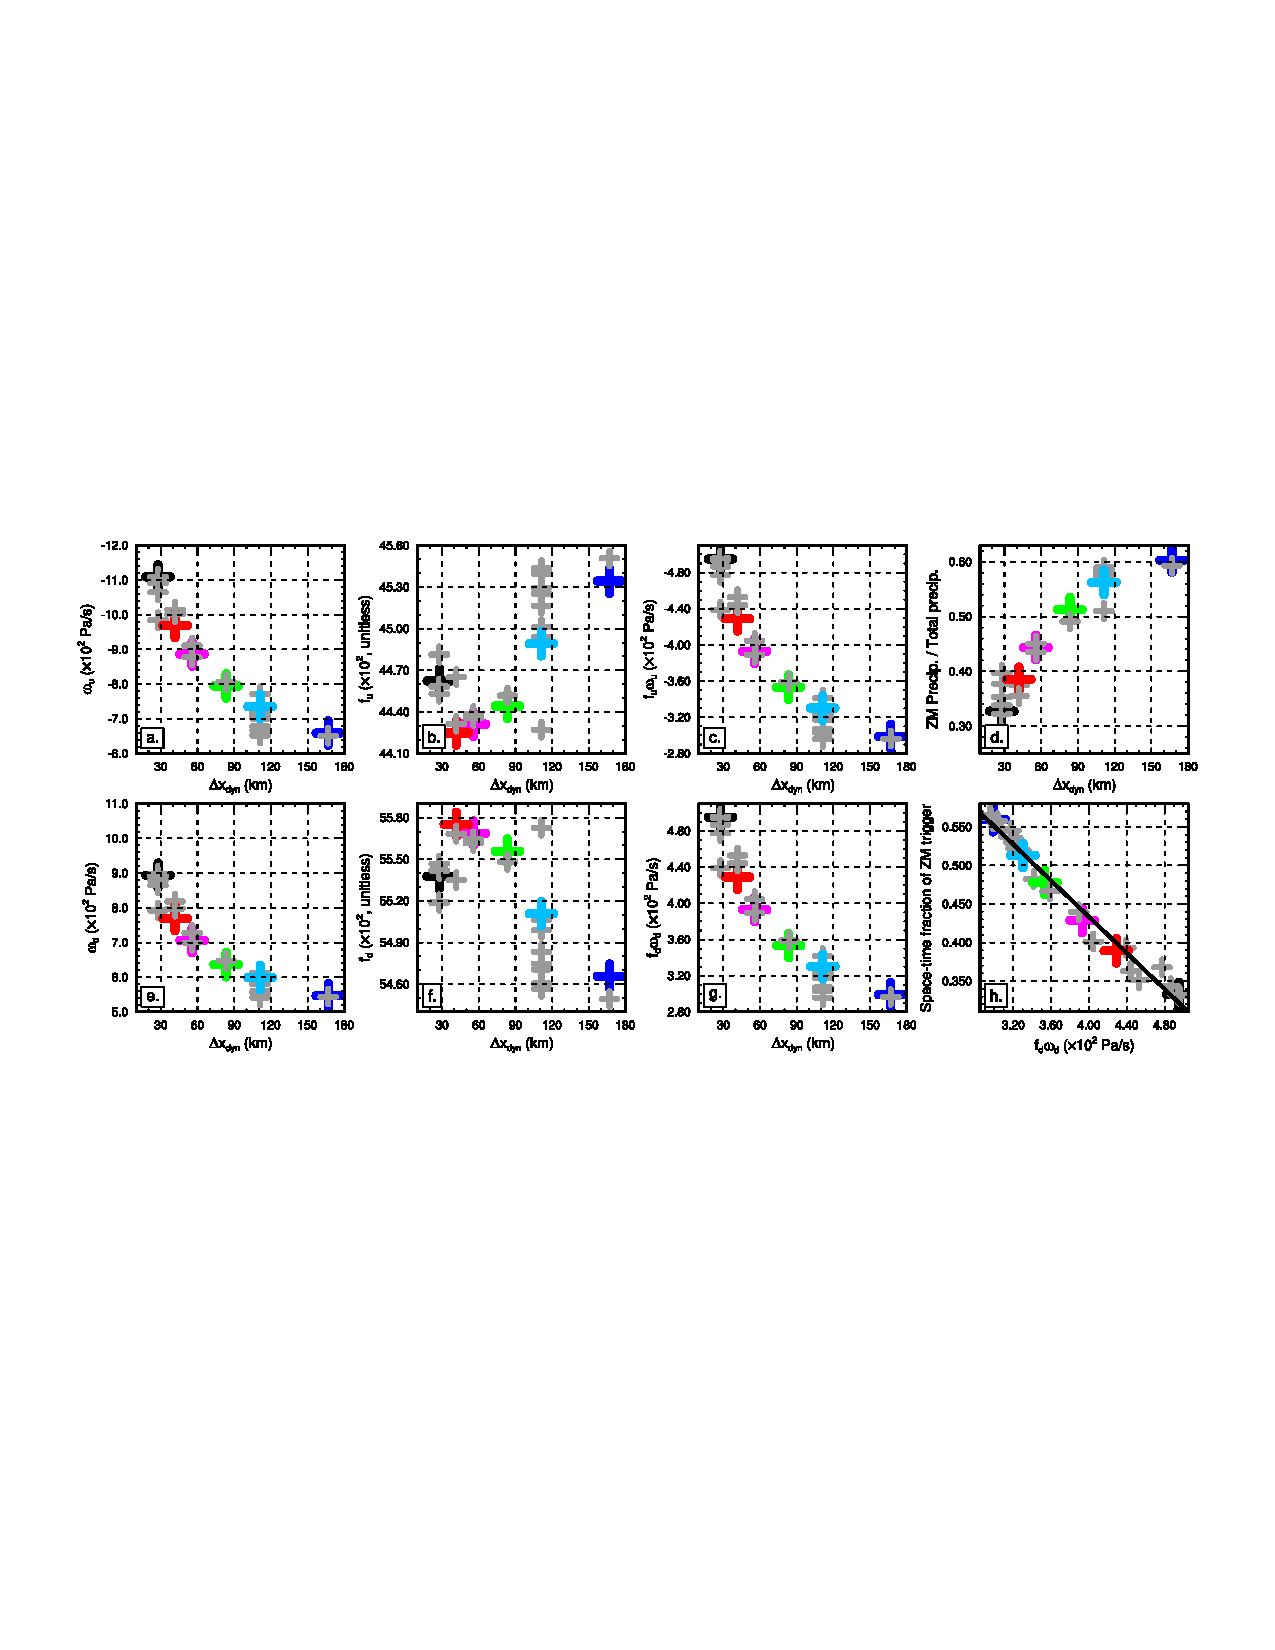
\includegraphics[width=40pc,angle=0]{chapter6/temp_diags_8panel.pdf}\\
\end{center}
\caption{}
\label{fig:8panel}
\end{figure}

As was mentioned in Section 6.1, it is common for the activity of deep convection scheme to become less active with increasing resolution in CAM. This is depicted in Figure~\ref{fig:8panel}d, which shows the global mean fraction of total precipitation arising from the deep convective scheme ({\em{ZM scheme}}) decreasing from about $0.60$ at low resolution ($ne20$) to about $0.32$ at high resolution ($ne120$). The global mean space time fraction the ZM scheme is triggered is highly negatively correlated with $\overline{\langle f_{d} \rangle} \, \overline{\langle \omega_{d} \rangle}$ in the 29 simulations (Pearson's R-value = 0.99; Figure~\ref{fig:8panel}h), more then with any individual component of equation~\ref{eq:eq6-2}. 

Obviously the same goodness of fit in Figure~\ref{fig:8panel}h is found using $\overline{\langle f_{u} \rangle} \, \overline{\langle \omega_{u} \rangle}$ as the predictor in the linear regression. To clear up this ambiguity, a logistic regression is performed on each grid column in the aqua-planets. Logistic regression uses an iterative method to fit a continuous variable predictor, $x$ to a binary predictand $p$ \citep{},
\begin{equation}
p = \frac{exp{[b_0 + b_1 x]}}{1 + exp{[b_0 + b_1 x]}}, \label{eq:eq6-3}
\end{equation}
where $b_0$ and $b_1$ are the shape parameters of the exponential. The predictor is chosen as the instantaneous $\langle f_{d} \rangle \langle \omega_{d} \rangle$ of a grid column, and the predictand is whether or not the ZM scheme is active, $1$ for yes and $0$ for no. Since the aqua-planets have zonally symmetric boundary conditions, there is a zonally varying structure in the goodness of fit (R-value) and the shape parameter $b_1$ (Figure~\ref{fig:4reg})a,b, with the largest R-values in the deep tropics and the high-latitudes. 

The R-value and the magnitude of $b_1$ decreases with increasing resolution, but everything shown is still statistically significant at the 95\% level using a likleihood ratio test \citep{}. The $b_1$ relationship between $\langle f_{d} \rangle \langle \omega_{d} \rangle$ and the ZM scheme is very large and negative in the deep tropics, where the ZM scheme is most active (not shown), indicating that greater downward motion in a grid column favors no deep convection. Repeating the regression using $\langle f_{u} \rangle \langle \omega_{u} \rangle$ as the predictor gives R-values that are generally less everywhere, especially in the deep tropics (not shown), and $b_1$ is still negative, and greater upward vertical motion favors deep convection.
The ZM trigger function is a dilute form of CAPE. In the classical, non-dilute case, CAPE can be broken into two main components; the instability of parcels in the boundary layer, influenced directly through surface fluxes, and instability due to the advection of dry static energy and moisture by the environment, i.e., the resolved flow. The latter generally results in an increase in CAPE in regions of ascent and a reduction in CAPE in regions of subsidence, which is consistent with our logistic regression producing a negative slope, $b_1$ between $\langle f_{d} \rangle \langle \omega_{d} \rangle$ and the activity of the ZM scheme.

\begin{figure}[t]
\begin{center}
\noindent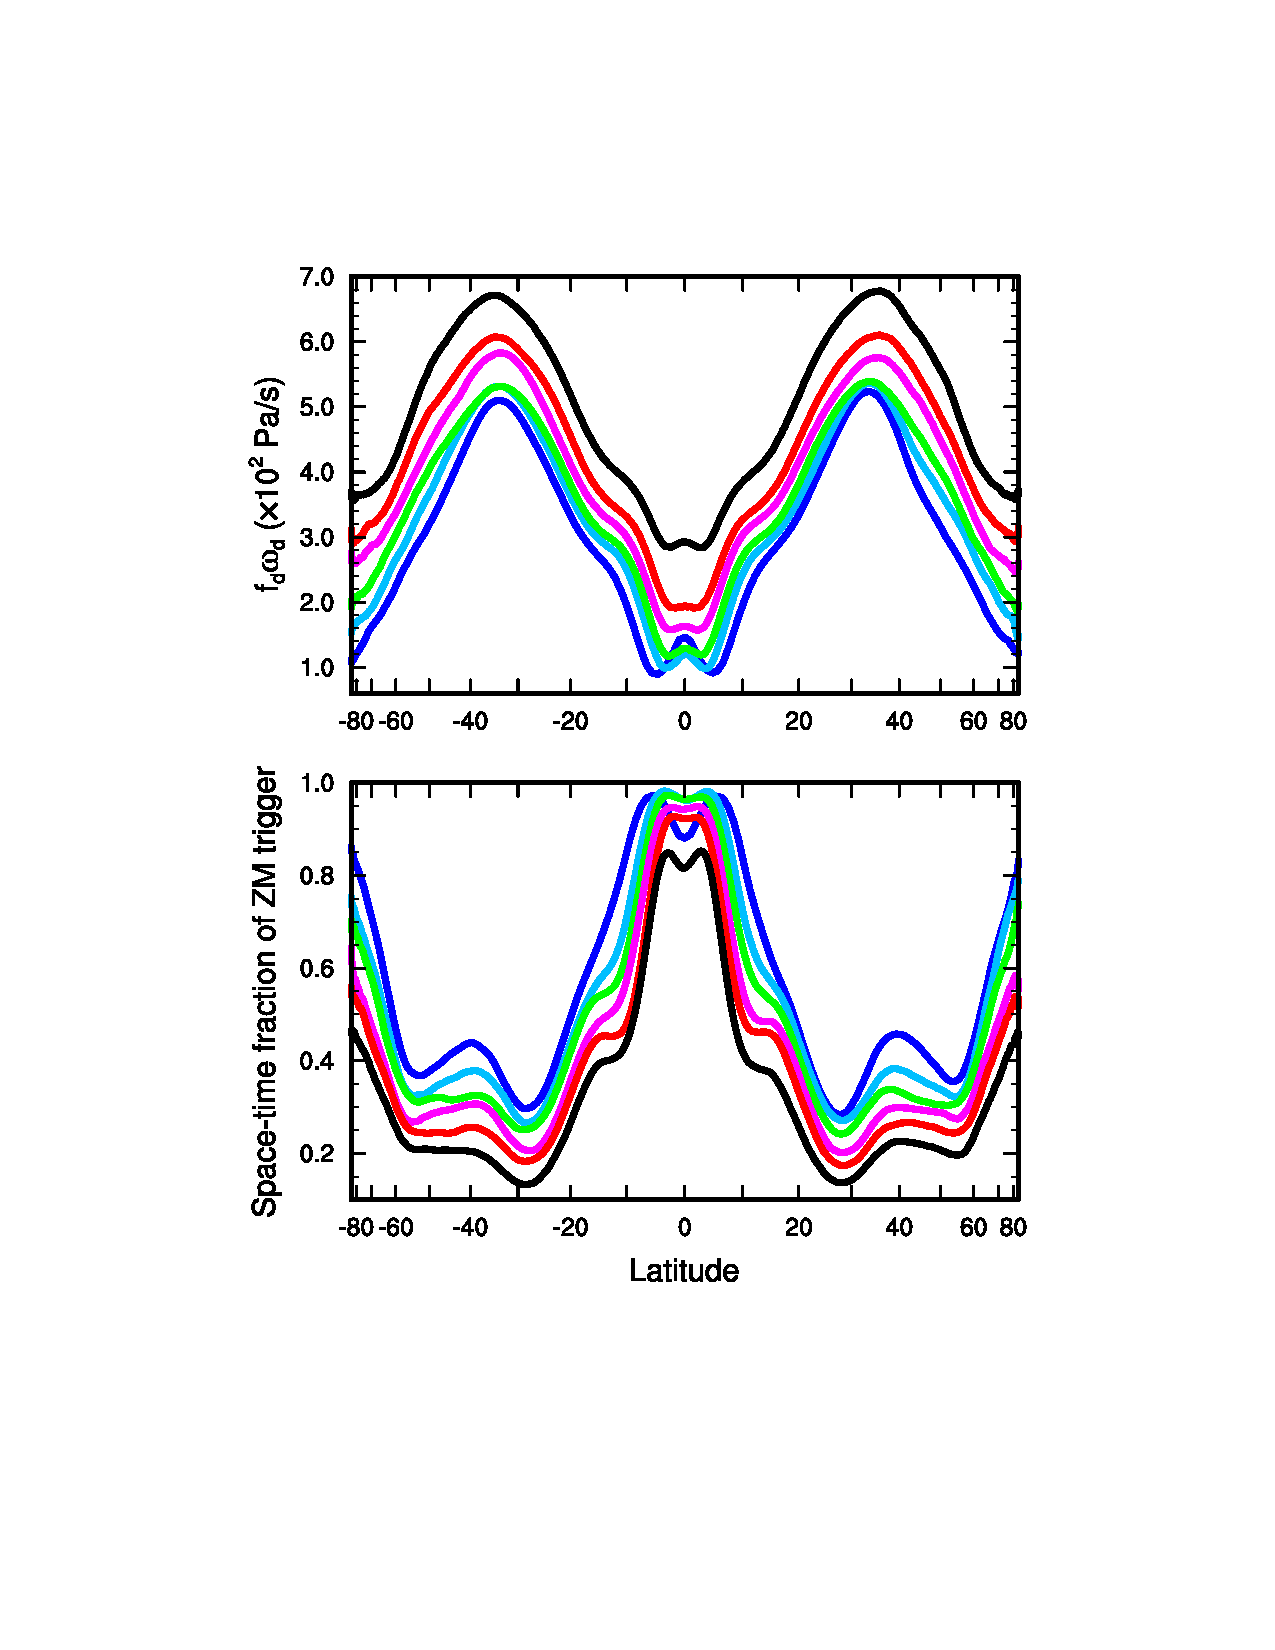
\includegraphics[width=20pc,angle=0]{chapter6/temp_zonal_fracd*vomgd.pdf}\\
\end{center}
\caption{}
\label{fig:vomg}
\end{figure}

Figure~\ref{fig:vomg} shows the time mean zonally averaged $\langle f_{d} \rangle \langle \omega_{d} \rangle$ and the frequency the ZM scheme is triggered. As expected from the global means (Figure~\ref{fig:8panel}h), the time mean zonal mean $\langle f_{d} \rangle \langle \omega_{d} \rangle$ increases with resolution. The ZM scheme is most active in the deep tropics ($-10^{\circ} to 10^{\circ}$ latitude), and while $\langle f_{d} \rangle \langle \omega_{d} \rangle$ is small, it's influence on convective activity is very large (Figure~\ref{fig:4reg}b).

\begin{figure}[t]
\begin{center}
\noindent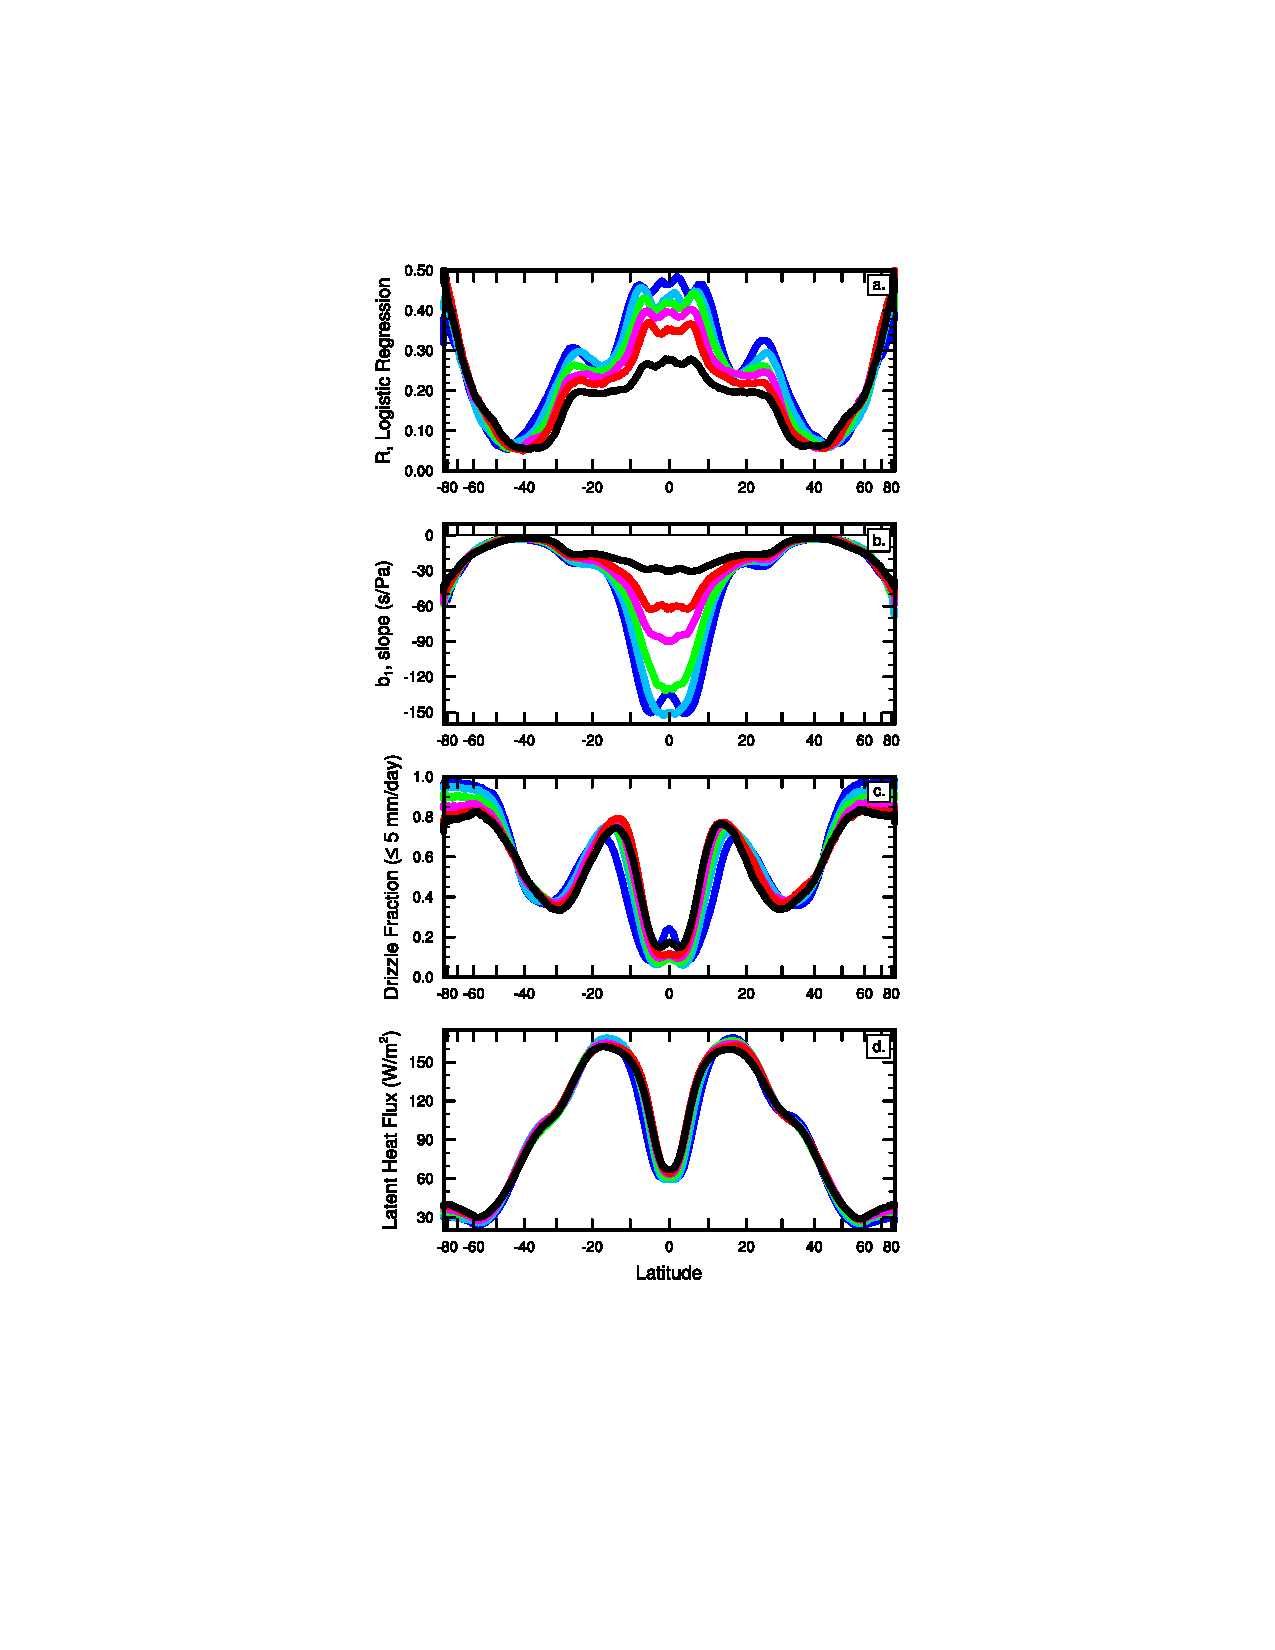
\includegraphics[width=14pc,angle=0]{chapter6/temp_zonal_4reg_dwn.pdf}\\
\end{center}
\caption{}
\label{fig:4reg}
\end{figure}

Polewards of $10^{\circ}$ latitude, $\langle f_{d} \rangle \langle \omega_{d} \rangle$ starts to increase, and the relationship between $\langle f_{d} \rangle \langle \omega_{d} \rangle$ and the ZM trigger reaches a local minimum at about $15^{\circ}$ (Figure~\ref{fig:4reg}b). Figure~\ref{fig:4reg}d shows the time mean zonal average latent heat fluxes, and indicates a maximum in the same region, about $10^{\circ}$. Between $10^{\circ} and 20^{\circ}$ the latent heat fluxes contribute to a positive CAPE while $\langle f_{d} \rangle \langle \omega_{d} \rangle$ is opposing CAPE, but unable to bring it below the trigger threshold of $70$ J/kg. The ZM precipitation associated with this region primarily consists of drizzle, shown in Figure~\ref{fig:4reg} as the fraction of convective precipitation rates $\leq 5$ mm/day relative to all convective precipitation rates. The drizzle fraction is known model bias in AGCMs, and is driven by two components of CAPE opposing one another. 

\begin{figure}[t]
\begin{center}
\noindent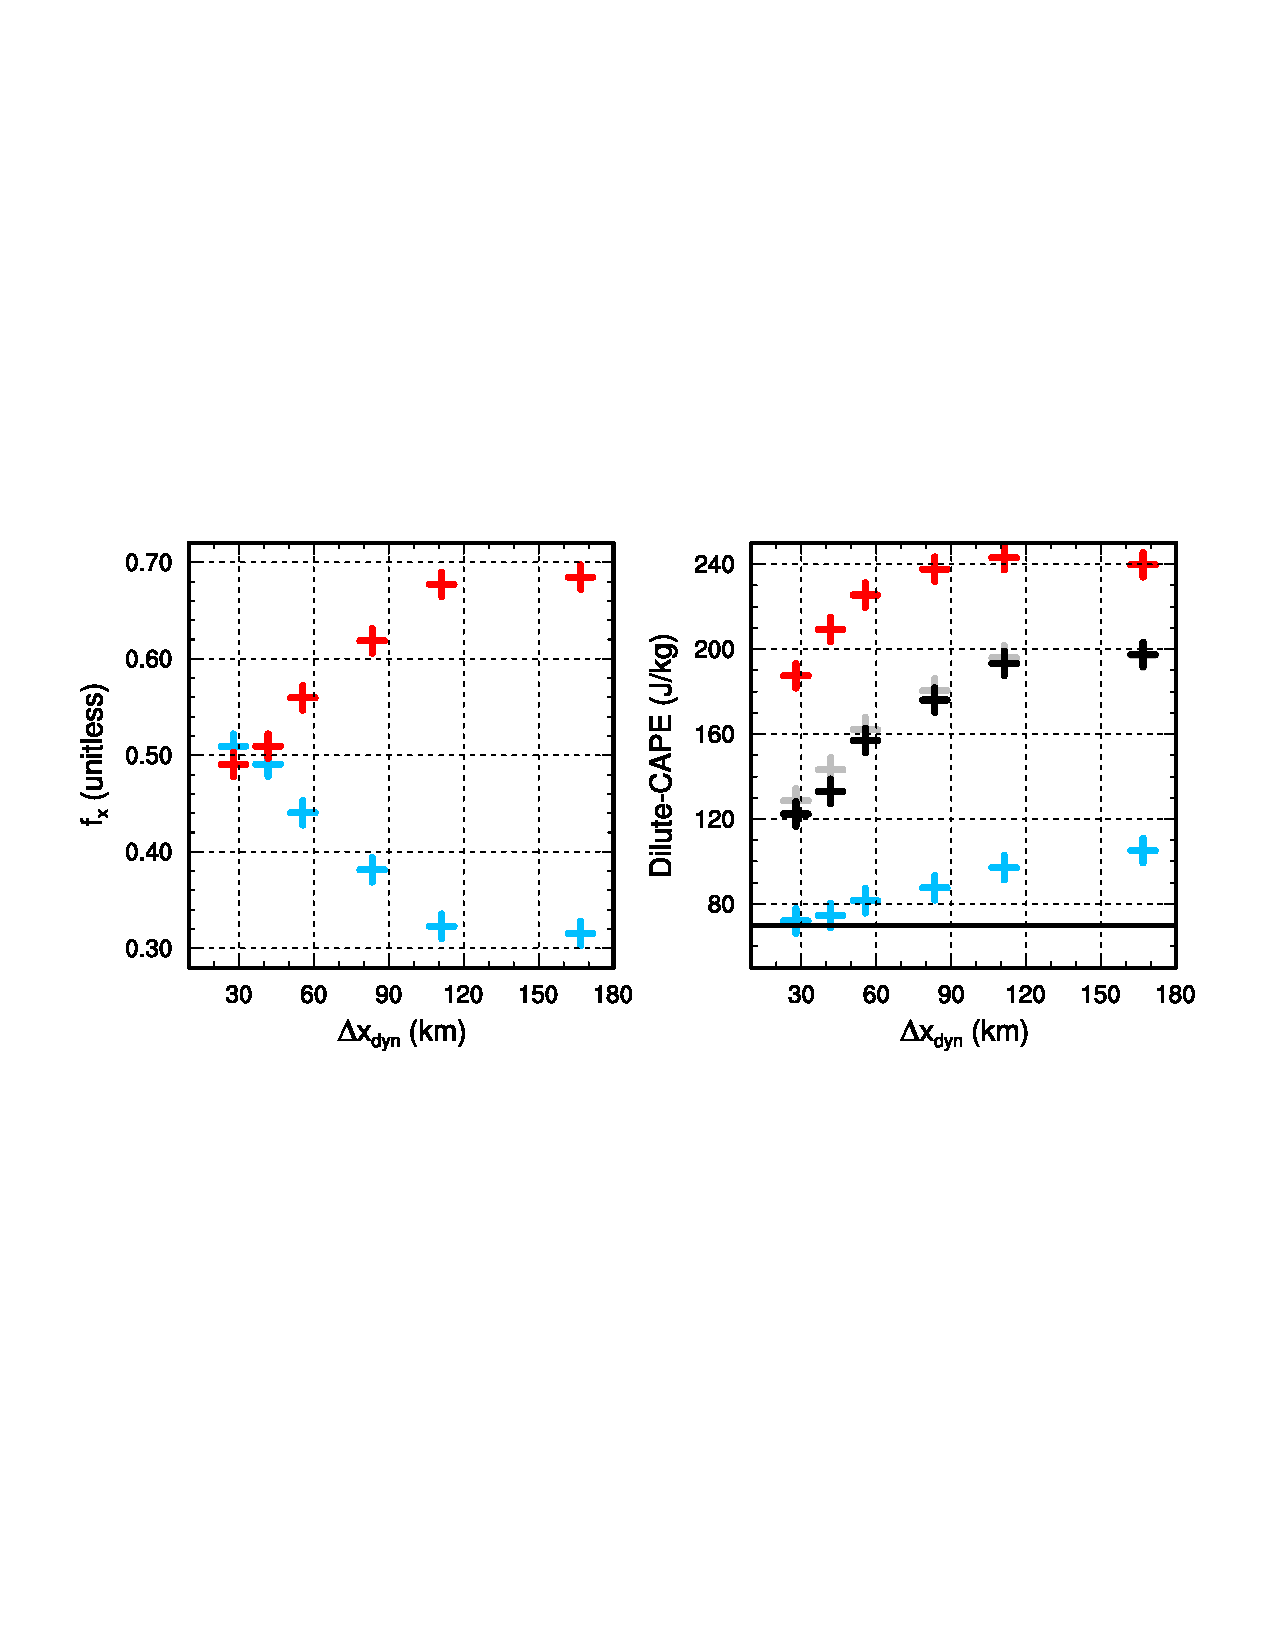
\includegraphics[width=25pc,angle=0]{chapter6/temp_cape.pdf}\\
\end{center}
\caption{}
\label{fig:cape}
\end{figure}